\subsection{Algoritmi na grafih}

\begin{naloga}{?}{Vaje OR 20.4.2016}
\begin{vprasanje}[matgraf]
Zasnuj podatkovno strukturo za grafe,
ki temelji na matrični predstavitvi.
Podatkovna struktura naj ima sledeče metode:
\begin{itemize}
\item {\tt \_\_init\_\_(G)}: ustvarjanje praznega grafa
\item {\tt dodajVozlisce(G, u)}: dodajanje novega vozlišča
\item {\tt dodajPovezavo(G, u, v)}: dodajanje nove povezave
\item {\tt brisiPovezavo(G, u, v)}: brisanje povezave
\item {\tt brisiVozlisce(G, u)}: brisanje vozlišča
\item {\tt sosedi(G, u)}: seznam sosedov danega vozlišča
\end{itemize}
Za vsako od naštetih metod podaj tudi njeno časovno zahtevnost
v odvisnosti od števila vozlišč, števila povezav in stopenj vhodnih vozlišč.
Oceni tudi prostorsko zahtevnost celotne strukture.
\end{vprasanje}
\begin{odgovor}
\end{odgovor}
\end{naloga}


\begin{naloga}{?}{Vaje OR 20.4.2016}
\begin{vprasanje}[sosgraf]
Zasnuj podatkovno strukturo za grafe,
ki temelji na seznamih sosedov.
Zapiši metode kot pri prejšnji strukturi
ter oceni njihovo časovno zahtevnost
in prostorsko zahtevnost celotne strukture.
\end{vprasanje}
\begin{odgovor}
\end{odgovor}
\end{naloga}


\begin{naloga}{?}{Vaje OR 20.4.2016}
\begin{vprasanje}
Kako moramo spremeniti strukturi
iz nalog~\nal{matgraf} in~\nal{sosgraf},
da bosta predstavljali digrafe?
\end{vprasanje}
\begin{odgovor}
\end{odgovor}
\end{naloga}


\begin{naloga}{?}{Vaje OR 20.4.2016}
\begin{vprasanje}
Napiši algoritem, ki za vhodni graf $G$ določi, ali ima trikotnik.
Katero podatkovno strukturo za grafe boš uporabil?
\end{vprasanje}
\begin{odgovor}
\end{odgovor}
\end{naloga}


\begin{naloga}{?}{Vaje OR 4.5.2016}
\begin{vprasanje}
Dan je digraf $D = (V, E)$.
Pravimo, da je vozlišče $v \in V$ {\em zvezda} digrafa $D$,
če ima izhodno povezavo do vseh ostalih vozlišč
in v digrafu $D$ ni drugih povezav.
Napiši algoritem, ki poišče zvezdo danega digrafa, če ta obstaja.
\end{vprasanje}
\begin{odgovor}
\end{odgovor}
\end{naloga}


\begin{naloga}{Janoš Vidali}{Vaje OR 30.11.2016}
\begin{vprasanje}[bfs]
Na grafu s slike~\fig{} izvedi iskanje v širino.
V primerih, ko imaš več ena\-ko\-vred\-nih izbir,
upoštevaj abecedni vrstni red.
Za vsako povezavo določi, ali se nahaja v drevesu iskanja v širino.

\begin{slika}
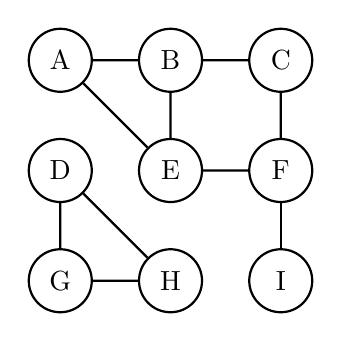
\begin{tikzpicture}[style=thick,scale=0.7]
\tikzstyle{vertex}=[draw, circle, fill=white, inner sep=0pt, minimum size=8mm]

\node[vertex] (A) at (-2, 2) {A};
\node[vertex] (B) at ( 0, 2) {B};
\node[vertex] (C) at ( 2, 2) {C};
\node[vertex] (D) at (-2, 0) {D};
\node[vertex] (E) at ( 0, 0) {E};
\node[vertex] (F) at ( 2, 0) {F};
\node[vertex] (G) at (-2,-2) {G};
\node[vertex] (H) at ( 0,-2) {H};
\node[vertex] (I) at ( 2,-2) {I};

\draw (B) -- (E) -- (A) -- (B) -- (C) -- (F) -- (E);
\draw (F) -- (I);
\draw (D) -- (G) -- (H) -- (D);
\end{tikzpicture}
\caption{Graf za nalogi~\nal{} in~\nal{dfs}.}
\end{slika}
\end{vprasanje}
\begin{odgovor}
\end{odgovor}
\end{naloga}


\begin{naloga}{?}{Vaje OR 4.5.2016}
\begin{vprasanje}
Zapiši algoritem, ki za vhodni graf $G$ določi njegov premer.

\end{vprasanje}
\begin{odgovor}
\end{odgovor}
\end{naloga}


\begin{naloga}{Janoš Vidali}{Vaje OR 7.12.2016}
\begin{vprasanje}[dijkstra]
S pomočjo Dijkstrovega algoritma
določi razdalje od vozlišča $A$ do ostalih vozlišč
v grafu s slike~\fig{}.

\begin{slika}
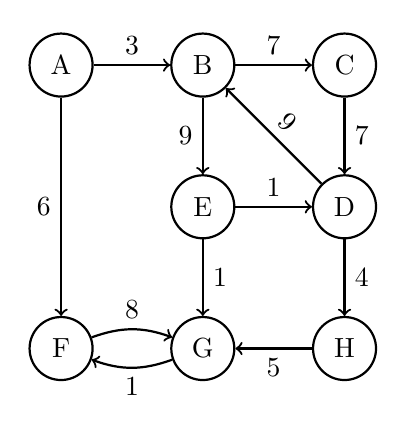
\begin{tikzpicture}[style=thick,scale=0.9]
\tikzstyle{vertex}=[draw, circle, fill=white, inner sep=0pt, minimum size=8mm]

\node[vertex] (A) at (-2, 2) {A};
\node[vertex] (B) at ( 0, 2) {B};
\node[vertex] (C) at ( 2, 2) {C};
\node[vertex] (D) at ( 2, 0) {D};
\node[vertex] (E) at ( 0, 0) {E};
\node[vertex] (F) at (-2,-2) {F};
\node[vertex] (G) at ( 0,-2) {G};
\node[vertex] (H) at ( 2,-2) {H};

\draw[->] (A) -- (B)
    node [above, midway] {$3$};
\draw[->] (A) -- (F)
    node [left, midway] {$6$};
\draw[->] (B) -- (C)
    node [above, midway] {$7$};
\draw[->] (B) -- (E)
    node [left, midway] {$9$};
\draw[->] (C) -- (D)
    node [right, midway] {$7$};
\draw[->] (D) -- (B)
    node [above, midway, sloped] {$9$};
\draw[->] (D) -- (H)
    node [right, midway] {$4$};
\draw[->] (E) -- (D)
    node [above, midway] {$1$};
\draw[->] (E) -- (G)
    node [right, midway] {$1$};
\draw[->] (F) to[bend left=20] node [above, midway] {$8$} (G);
\draw[->] (G) to[bend left=20] node [below, midway] {$1$} (F);
\draw[->] (H) -- (G)
    node [below, midway] {$5$};
\end{tikzpicture}
\podnaslov{Graf}
\end{slika}
\end{vprasanje}
\begin{odgovor}
\end{odgovor}
\end{naloga}

\begin{naloga}{?}{Vaje OR 4.5.2016}
\begin{vprasanje}
Naj bo $G = (V, E)$ graf,
za katerega so dolžine povezav določene s funkcijo $\ell : E \to \R$
(tj., dolžine so lahko tudi negativne).
Definirajmo še funkcijo $\ell' : E \to \R$ tako,
da velja $\ell'(e) = \ell(e) - \min\set{\ell(f)}{f \in E}$
(dolžine, določene z $\ell'$, so torej nenegativne).
Dokaži ali ovrzi: drevo najkrajših poti,
ki ga Dijkstrov algoritem ustvari ob vhodu $(G, \ell')$,
je tudi drevo najkrajših poti za graf $G$ z dolžinami povezav,
določenimi z $\ell$.
\end{vprasanje}
\begin{odgovor}
\end{odgovor}
\end{naloga}


\begin{naloga}%
{Dasgupta, Papadimitriou, Vazirani}{\cite[Exercise~4.13]{dpv}}
\begin{vprasanje}
Denimo, da imamo neusmerjen graf $G = (V, E)$,
katerega vozlišča pred\-stav\-lja\-jo mesta,
povezave pa predstavljajo ceste, ki jih povezujejo.
Za vsako povezavo $e \in E$ poznamo njeno dolžino $\ell_e$ (v kilometrih).

Priti želimo iz mesta $s$ v mesto $t$.
V vsakem mestu je bencinska črpalka, ob cestah pa teh ni.
Žal imamo na voljo samo star avto,
ki lahko s polnim rezervoarjem prepelje le $L$ kilometrov.
\begin{enumerate}[(a)]
\item Zapiši algoritem, ki v linearnem času poišče pot,
ki jo lahko prevozimo z našim avtom,
oziroma ugotovi, da ta ne obstaja.
\item Izkaže se, da z našim avtom te poti ne moremo prevoziti,
zato se odločimo za nakup novega.
Zapiši algoritem, ki v času $O(m \log n)$
določi najmanjše število prevoženih kilometrov,
ki naj jih avto zmore z enim polnjenjem,
da bo pot od $s$ do $t$ mogoča.
\end{enumerate}

\end{vprasanje}
\begin{odgovor}
\end{odgovor}
\end{naloga}


\begin{naloga}{Sergio Cabello}{Vaje OR 7.12.2016}
\begin{vprasanje}
Zasnuj različico Dijkstrovega algoritma
za iskanje najkrajše poti med vozliščema $s$ in $t$ v grafu $G$,
ki iskanje hkrati začne v vozliščih $s$ in $t$.
Kdaj naj se iskanje konča in kako naj se poišče rešitev?
\end{vprasanje}
\begin{odgovor}
\end{odgovor}
\end{naloga}


\begin{naloga}%
{Dasgupta, Papadimitriou, Vazirani}{\cite[Exercise~3.1]{dpv}}
\begin{vprasanje}[dfs]
Na grafu s slike~\fig{bfs} izvedi iskanje v globino.
V primerih, ko imaš več ena\-ko\-vred\-nih izbir,
upoštevaj abecedni vrstni red.
Za vsako povezavo določi, ali se nahaja v drevesu iskanja v globino.
\end{vprasanje}
\begin{odgovor}
\end{odgovor}
\end{naloga}


\begin{naloga}{Janoš Vidali}{Vaje OR 21.5.2018}
\begin{vprasanje}[bf]
S pomočjo Bellman-Fordovega algoritma
določi razdalje od vozlišča $A$ do ostalih vozlišč
v grafu s slike~\fig{}.

\begin{slika}
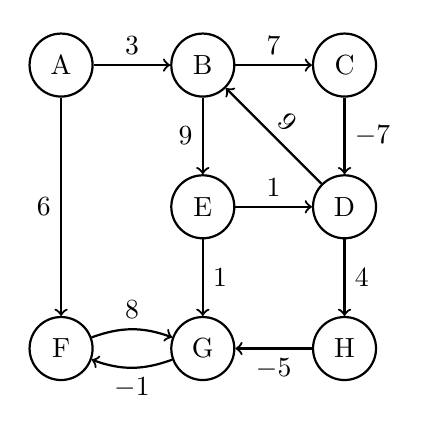
\begin{tikzpicture}[style=thick,scale=0.9]
\tikzstyle{vertex}=[draw, circle, fill=white, inner sep=0pt, minimum size=8mm]

\node[vertex] (A) at (-2, 2) {A};
\node[vertex] (B) at ( 0, 2) {B};
\node[vertex] (C) at ( 2, 2) {C};
\node[vertex] (D) at ( 2, 0) {D};
\node[vertex] (E) at ( 0, 0) {E};
\node[vertex] (F) at (-2,-2) {F};
\node[vertex] (G) at ( 0,-2) {G};
\node[vertex] (H) at ( 2,-2) {H};

\draw[->] (A) -- (B)
    node [above, midway] {$3$};
\draw[->] (A) -- (F)
    node [left, midway] {$6$};
\draw[->] (B) -- (C)
    node [above, midway] {$7$};
\draw[->] (B) -- (E)
    node [left, midway] {$9$};
\draw[->] (C) -- (D)
    node [right, midway] {$-7$};
\draw[->] (D) -- (B)
    node [above, midway, sloped] {$9$};
\draw[->] (D) -- (H)
    node [right, midway] {$4$};
\draw[->] (E) -- (D)
    node [above, midway] {$1$};
\draw[->] (E) -- (G)
    node [right, midway] {$1$};
\draw[->] (F) to[bend left=20] node [above, midway] {$8$} (G);
\draw[->] (G) to[bend left=20] node [below, midway] {$-1$} (F);
\draw[->] (H) -- (G)
    node [below, midway] {$-5$};
\end{tikzpicture}
\podnaslov{Graf}
\end{slika}
\end{vprasanje}
\begin{odgovor}
\end{odgovor}
\end{naloga}


\begin{naloga}{Janoš Vidali}{Vaje OR 7.12.2016}
\begin{vprasanje}[topo]
Dan je usmerjen acikličen graf s slike~\fig{}.

\begin{enumerate}[(a)]
\item Poišči topološko ureditev vozlišč zgornjega grafa.

\item Poišči najkrajšo pot od vozlišča $G$ do vozlišča $E$.

\item Poišči najdaljšo pot od vozlišča $G$ do vozlišča $E$.
\end{enumerate}

\begin{slika}
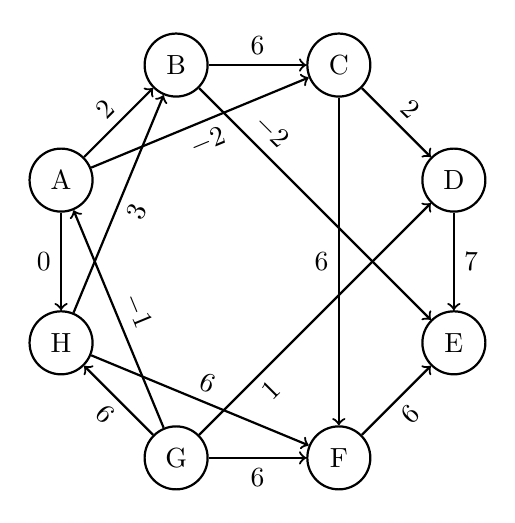
\begin{tikzpicture}[style=thick,scale=0.9]
\tikzstyle{vertex}=[draw, circle, fill=white, inner sep=0pt, minimum size=8mm]

\node[vertex] (A) at (xyz polar cs:angle=157.5,radius=3) {A};
\node[vertex] (B) at (xyz polar cs:angle=112.5,radius=3) {B};
\node[vertex] (C) at (xyz polar cs:angle= 67.5,radius=3) {C};
\node[vertex] (D) at (xyz polar cs:angle= 22.5,radius=3) {D};
\node[vertex] (E) at (xyz polar cs:angle=337.5,radius=3) {E};
\node[vertex] (F) at (xyz polar cs:angle=292.5,radius=3) {F};
\node[vertex] (G) at (xyz polar cs:angle=247.5,radius=3) {G};
\node[vertex] (H) at (xyz polar cs:angle=202.5,radius=3) {H};

\draw[->] (A) -- (B) node [above, midway, sloped] {$2$};
\draw[->] (A) -- (C) node [below, midway, sloped] {$-2$};
\draw[->] (A) -- (H) node [left, midway] {$0$};
\draw[->] (B) -- (C) node [above, midway] {$6$};
\draw[->] (B) -- (E) node [above, near start, sloped] {$-2$};
\draw[->] (C) -- (D) node [above, midway, sloped] {$2$};
\draw[->] (C) -- (F) node [left, midway] {$6$};
\draw[->] (D) -- (E) node [right, midway] {$7$};
\draw[->] (F) -- (E) node [below, midway, sloped] {$6$};
\draw[->] (G) -- (A) node [above, midway, sloped] {$-1$};
\draw[->] (G) -- (D) node [below, near start, sloped] {$1$};
\draw[->] (G) -- (F) node [below, midway] {$6$};
\draw[->] (G) -- (H) node [below, midway, sloped] {$6$};
\draw[->] (H) -- (B) node [below, midway, sloped] {$3$};
\draw[->] (H) -- (F) node [above, midway, sloped] {$6$};
\end{tikzpicture}
\podnaslov{Graf}
\end{slika}
\end{vprasanje}
\begin{odgovor}
\end{odgovor}
\end{naloga}


\begin{naloga}{?}{Kolokvij OR 9.5.2013}
\begin{vprasanje}[oviratlon]
Oviratlon je tekalna preizkušnja
na 8 do 10 kilometrov dolgi poti z različnimi ovirami.
Zanima nas, na koliko različnih načinov lahko pridemo od štarta do cilja.
Dan je utežen usmerjen acikličen graf $G$ ter vozlišči $s$ in $t$,
ki predstavljata štart oziroma cilj.
Uteži na povezavah nam predstavljajo,
na koliko načinov jih lahko prečkamo.

\begin{enumerate}[(a)]
\item Reši nalogo za graf s slike~\fig{}.

\item Zapiši algoritem, ki reši dani problem.
Kakšna je njegova časovna zahtevnost?
\end{enumerate}

\begin{slika}
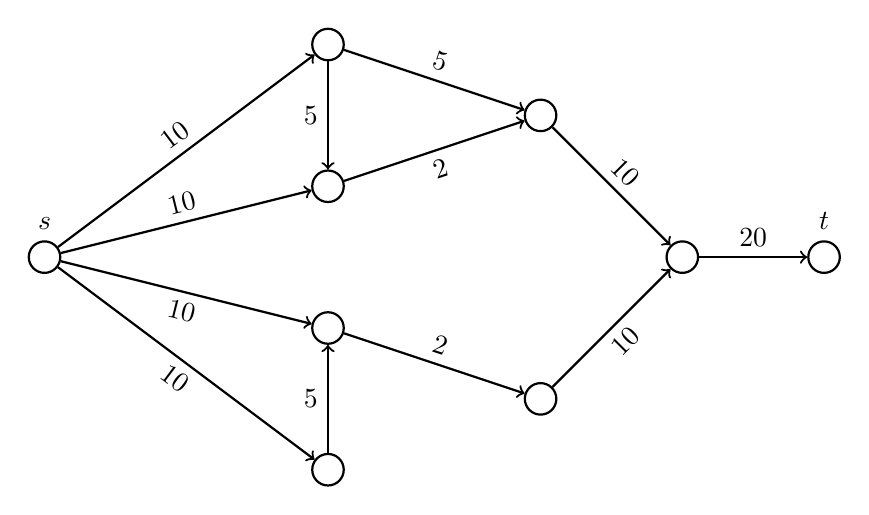
\begin{tikzpicture}[style=thick,scale=0.9]
\tikzstyle{vertex}=[draw, circle, fill=white, inner sep=0pt, minimum size=4mm]

\node[vertex] (S) at (-5, 0) [label=above:$s$] {};
\node[vertex] (A) at (-1, 3) {};
\node[vertex] (B) at (-1, 1) {};
\node[vertex] (C) at (-1,-1) {};
\node[vertex] (D) at (-1,-3) {};
\node[vertex] (E) at ( 2, 2) {};
\node[vertex] (F) at ( 2,-2) {};
\node[vertex] (G) at ( 4, 0) {};
\node[vertex] (T) at ( 6, 0) [label=above:$t$] {};

\draw[->] (S) -- (A)
    node [above, midway, sloped] {$10$};
\draw[->] (S) -- (B)
    node [above, midway, sloped] {$10$};
\draw[->] (S) -- (C)
    node [below, midway, sloped] {$10$};
\draw[->] (S) -- (D)
    node [below, midway, sloped] {$10$};
\draw[->] (A) -- (B)
    node [left, midway] {$5$};
\draw[->] (A) -- (E)
    node [above, midway, sloped] {$5$};
\draw[->] (B) -- (E)
    node [below, midway, sloped] {$2$};
\draw[->] (C) -- (F)
    node [above, midway, sloped] {$2$};
\draw[->] (D) -- (C)
    node [left, midway] {$5$};
\draw[->] (E) -- (G)
    node [above, midway, sloped] {$10$};
\draw[->] (F) -- (G)
    node [below, midway, sloped] {$10$};
\draw[->] (G) -- (T)
    node [above, midway] {$20$};

\end{tikzpicture}
\podnaslov{Graf}
\end{slika}
\end{vprasanje}
\begin{odgovor}
\end{odgovor}
\end{naloga}


\begin{naloga}{Janoš Vidali}{Izpit OR 15.12.2016}
\begin{vprasanje}[zaklad]
Lovec na zaklade se z bogatim ulovom
vrača iz Kalifornije nazaj domov v Chicago,
pri čemer mora seveda prečkati Divji zahod.
Potoval bo s kočijo,
pri čemer bo vsak dan potoval med dvema mestoma in nato prespal.
Zaradi varnosti se bo držal samo državnih cest, ki so varne.
Toda mesta, kjer bo prespal, niso povsem varna.
Za vsako mesto pozna verjetnosti,
da ga tam ne bodo oropali (te so med seboj neodvisne).
Tako bi želel načrtovati najvarnejšo pot domov
-- torej pot z največjo verjetnostjo,
da ga pri nobenem postanku ne bodo oropali.

\begin{enumerate}[(a)]
\item Mesta in ceste med njimi lahko predstavimo z vozlišči in povezavami
v ne\-usme\-rje\-nem grafu $G$, verjetnosti pa kot teže vozlišč.
Opiši, kako lahko za dani graf $G$ z uteženimi vozlišči
učinkovito poiščemo ustrezno pot med danima vozliščema $s$ in $t$
z uporabo variante Dijkstrovega algoritma,
ter utemelji njegovo ustreznost.
Lahko predpostaviš, da sta teži začetnega in končnega vozlišča enaki $1$.

\item Reši problem za graf s slike~\fig{},
pri čemer naj se pot začne v LA in konča v CH.
Zadostovalo bo, če verjetnosti računaš na $3$ decimalke natančno.
\end{enumerate}

\begin{slika}
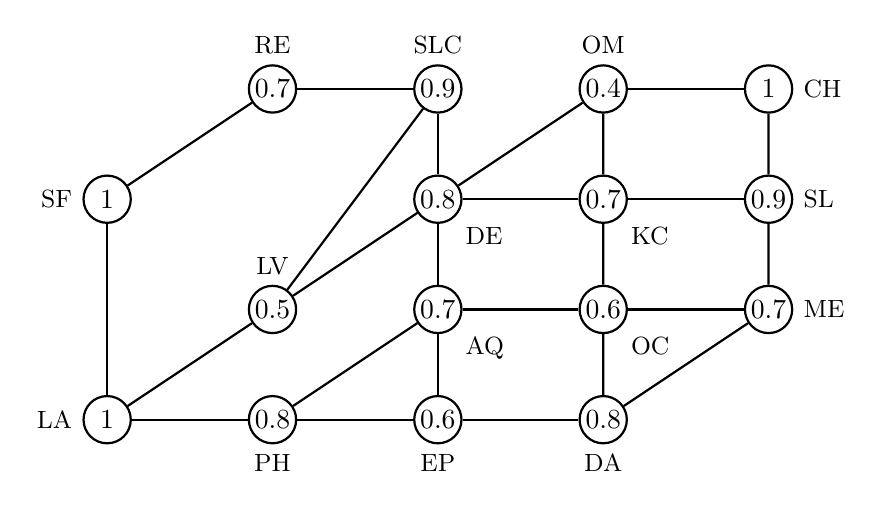
\begin{tikzpicture}[style=thick,scale=0.7]
\tikzstyle{every node}=[]
\tikzstyle{vertex}=[draw, circle, inner sep=-2pt, minimum size=6mm]

\node[vertex] (ns) at (-6,-3) [label=left: {\small LA} ] {$1$};
\node[vertex] (na) at (-6, 1) [label=left: {\small SF} ] {$1$};
\node[vertex] (nb) at (-3,-3) [label=below:{\small PH} ] {$0.8$};
\node[vertex] (nc) at (-3,-1) [label=above:{\small LV} ] {$0.5$};
\node[vertex] (nd) at (-3, 3) [label=above:{\small RE} ] {$0.7$};
\node[vertex] (ne) at ( 0,-3) [label=below:{\small EP} ] {$0.6$};
\node[vertex] (nf) at ( 0,-1) [label=315:  {\small AQ} ] {$0.7$};
\node[vertex] (ng) at ( 0, 1) [label=315:  {\small DE} ] {$0.8$};
\node[vertex] (nh) at ( 0, 3) [label=above:{\small SLC}] {$0.9$};
\node[vertex] (ni) at ( 3,-3) [label=below:{\small DA} ] {$0.8$};
\node[vertex] (nj) at ( 3,-1) [label=315:  {\small OC} ] {$0.6$};
\node[vertex] (nk) at ( 3, 1) [label=315:  {\small KC} ] {$0.7$};
\node[vertex] (nl) at ( 3, 3) [label=above:{\small OM} ] {$0.4$};
\node[vertex] (nm) at ( 6,-1) [label=right:{\small ME} ] {$0.7$};
\node[vertex] (nn) at ( 6, 1) [label=right:{\small SL} ] {$0.9$};
\node[vertex] (nt) at ( 6, 3) [label=right:{\small CH} ] {$1$};

\draw (ns) -- (na);
\draw (ns) -- (nb);
\draw (ns) -- (nc);
\draw (na) -- (nd);
\draw (nb) -- (ne);
\draw (nb) -- (nf);
\draw (nc) -- (ng);
\draw (nc) -- (nh);
\draw (nd) -- (nh);
\draw (ne) -- (nf);
\draw (ne) -- (ni);
\draw (nf) -- (ng);
\draw (nf) -- (nj);
\draw (ng) -- (nh);
\draw (ng) -- (nk);
\draw (ng) -- (nl);
\draw (ni) -- (nj);
\draw (ni) -- (nm);
\draw (nj) -- (nk);
\draw (nj) -- (nm);
\draw (nk) -- (nl);
\draw (nk) -- (nn);
\draw (nl) -- (nt);
\draw (nm) -- (nn);
\draw (nn) -- (nt);
\end{tikzpicture}
\podnaslov{Graf}
\end{slika}
\end{vprasanje}
\begin{odgovor}
\end{odgovor}
\end{naloga}


\begin{naloga}{Sergio Cabello}{Izpit OR 15.3.2017}
\begin{vprasanje}
Dan je usmerjen graf $G = (V, E)$ s pozitivnimi dolžinami povezav.
Dano imamo še vozlišče $s \in V$
ter vrednost $\delta_v$ za vsako vozlišče $v \in V$.
Natančno opiši algoritem (z besedami ali psevdokodo),
ki v času $O(m)$ (kjer je $m = |V| + |E|$) preveri,
ali velja $\delta_v = d_G(s, v)$ za vse $v \in V$
-- t.j., v linearnem času preveri,
ali so vrednosti $\delta_v$
enake razdalji med vozliščema $s$ in $v$ v grafu $G$.

Lahko predpostaviš, da so vsa vozlišča grafa $G$ dosegljiva iz vozlišča $s$.
Utemelji pravilnost meje za časovno zahtevnost algoritma.
\end{vprasanje}
\begin{odgovor}
\end{odgovor}
\end{naloga}


\begin{naloga}{Janoš Vidali}{Izpit OR 10.7.2017}
\begin{vprasanje}[pocitnice]
Z električnim vozilom se odpravljamo na počitnice.
Vozilo moramo vsako noč napolniti,
zato smo si pripravili seznam krajev in cestnih povezav med njimi,
ki jih lahko prevozimo v enem dnevu.
Poiskati želimo pot od začetne točke do destinacije,
ki bo imela čim manjše število postankov (tj., bo trajala čim manj dni).

\begin{enumerate}[(a)]
\item Predstavi problem v jeziku grafov
in predlagaj algoritem za njegovo reševanje.

\item Na koncu počitnic razmišljamo o poti nazaj.
Spet bi radi naredili čim manj postankov,
a se pri tem ne želimo ustaviti v nobenem kraju,
kjer smo se ustavili na poti naprej.
Dopolni zgornji algoritem, da bo našel še ustrezno pot nazaj.

\item S pomočjo zgornjih algoritmov poišči najkrajšo pot od LJ do AM
in najkrajšo pot nazaj v grafu s slike~\fig{},
ki ne gre čez kraje iz prejšnje poti.
\end{enumerate}

\begin{slika}
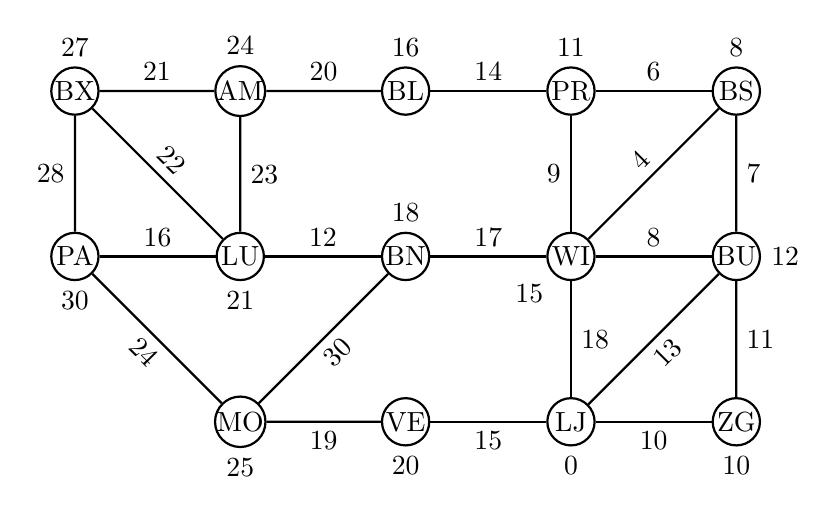
\begin{tikzpicture}[style=thick,scale=0.7]
\tikzstyle{every node}=[]
\tikzstyle{vertex}=[draw, circle, fill=white, inner sep=0pt, minimum size=6mm]

\node[vertex] (ns) at ( 3,-3) [label=below:$0$ ] {LJ};
\node[vertex] (na) at ( 6,-3) [label=below:$10$] {ZG};
\node[vertex] (nb) at ( 0,-3) [label=below:$20$] {VE};
\node[vertex] (nc) at (-3,-3) [label=below:$25$] {MO};
\node[vertex] (nd) at ( 6, 0) [label=right:$12$] {BU};
\node[vertex] (ne) at ( 3, 0) [label=  225:$15$] {WI};
\node[vertex] (nf) at ( 0, 0) [label=above:$18$] {BN};
\node[vertex] (ng) at (-3, 0) [label=below:$21$] {LU};
\node[vertex] (nh) at (-6, 0) [label=below:$30$] {PA};
\node[vertex] (ni) at ( 6, 3) [label=above:$8$ ] {BS};
\node[vertex] (nj) at ( 3, 3) [label=above:$11$] {PR};
\node[vertex] (nk) at ( 0, 3) [label=above:$16$] {BL};
\node[vertex] (nl) at (-6, 3) [label=above:$27$] {BX};
\node[vertex] (nt) at (-3, 3) [label=above:$24$] {AM};

\draw (ns) -- (na) node[below, midway]         {$10$};
\draw (ns) -- (nb) node[below, midway]         {$15$};
\draw (ns) -- (nd) node[below, midway, sloped] {$13$};
\draw (ns) -- (ne) node[right, midway]         {$18$};
\draw (na) -- (nd) node[right, midway]         {$11$};
\draw (nb) -- (nc) node[below, midway]         {$19$};
\draw (nc) -- (nf) node[below, midway, sloped] {$30$};
\draw (nc) -- (nh) node[below, midway, sloped] {$24$};
\draw (nd) -- (ne) node[above, midway]         {$8$};
\draw (nd) -- (ni) node[right, midway]         {$7$};
\draw (ne) -- (nf) node[above, midway]         {$17$};
\draw (ne) -- (ni) node[above, midway, sloped] {$4$};
\draw (ne) -- (nj) node[left, midway]          {$9$};
\draw (nf) -- (ng) node[above, midway]         {$12$};
\draw (ng) -- (nh) node[above, midway]         {$16$};
\draw (ng) -- (nl) node[above, midway, sloped] {$22$};
\draw (ng) -- (nt) node[right, midway]         {$23$};
\draw (nh) -- (nl) node[left, midway]          {$28$};
\draw (ni) -- (nj) node[above, midway]         {$6$};
\draw (nj) -- (nk) node[above, midway]         {$14$};
\draw (nk) -- (nt) node[above, midway]         {$20$};
\draw (nl) -- (nt) node[above, midway]         {$21$};
\end{tikzpicture}
\caption{Graf za nalogi~\nal{} (brez uteži) in~\nal{pot}.}
\end{slika}
\end{vprasanje}
\begin{odgovor}
\end{odgovor}
\end{naloga}


\begin{naloga}{Janoš Vidali}{Kolokvij OR 11.6.2018}
\begin{vprasanje}[prerezna]
Dan je povezan neusmerjen enostaven graf $G = (V, E)$
(tj., brez zank in večkratnih povezav).
{\em Prerezno vozlišče} v grafu $G$ je tako vozlišče $u \in V$,
da graf $G - u$
(tj., graf $G$ brez vozlišča $u$ in povezav s krajiščem v $u$)
ni več povezan.
Poiskati želimo seznam prereznih vozlišč grafa $G$.

Pri iskanju si bomo pomagali s preiskovanjem v globino.
Ob prvem obisku vozlišča $u$ s predhodnikom $v$
se tako pokliče funkcija \verb|previsit(u, v)|,
ob njegovem zadnjem obisku pa funkcija \verb|postvisit(u, v)|.
Če je $u$ koren preiskovalnega drevesa, potem ima $v$ vrednost \verb|None|.
Predpostavi, da imaš v obeh funkcijah dostop do seznama \verb|izhod|,
kamor bo treba dodati najdena presečna vozlišča.
Prav tako imata lahko obe funkciji dostop do drugih pomožnih spremenljivk.

Naj bo $\ell_u$ globina vozlišča $u$ v drevesu iskanja v globino
(tj., razdalja od korena do $u$ v drevesu iskanja v globino).
Za vsako vozlišče $u$ definiramo vrednost $p_u$ kot najmanjšo globino vozlišč,
ki so v grafu $G$ sosedna vozlišču $u$
ali njegovim potomcem v drevesu iskanja v globino.

\begin{enumerate}[(a)]
\item Za graf na sliki~\fig{} nariši drevo iskanja v globino
(v njem označi tudi povratne povezave, npr.~s črtkano črto)
in določi njegova prerezna vozlišča.
Upoštevaj abecedni vrstni red obiskovanja vozlišč.
Za vsako vozlišče $u$ določi še vrednosti $\ell_u$ in $p_u$. \\
{\small {\bf Namig:}
vrednosti $p_u$ najprej določi za vozlišča z večjo globino.}

\item Napiši rekurzivno formulo za vrednost $p_u$. \\
{\small {\bf Namig:} loči med sosedi $v$ vozlišča $u$ v grafu $G$
(pišeš lahko $u \sim v$)
in njegovimi neposrednimi nasledniki $w$ v preiskovalnem drevesu ($u \to w$).}

\item Natančno opiši funkcijo \verb|previsit(u, v)|
(z besedami ali psevdokodo),
ki poskrbi za izračun vrednosti $\ell_u$.

\item Natančno opiši funkcijo \verb|postvisit(u, v)|
(z besedami ali psevdokodo),
ki naj za vozlišče $u$ izračuna vrednost $p_u$ in ugotovi,
ali je $u$ prerezno vozlišče, in ga v tem primeru doda v \verb|izhod|.
Predpostavi, da imaš globine vozlišč že poračunane
(tudi, če točka (c) ni rešena). \\
{\small {\bf Namig:} obravnavaj dve možnosti --
ko je $u$ koren drevesa, in ko $u$ ni koren drevesa.
Kako v vsakem od teh primerov ugotoviš, ali je $u$ prerezno vozlišče?}

\item Oceni časovno zahtevnost celotnega algoritma.
\end{enumerate}

\begin{slika}
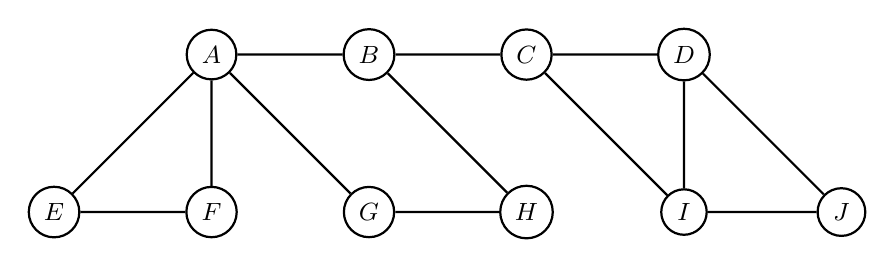
\begin{tikzpicture}[style=thick,scale=2]
\tikzstyle{vertex}=[draw, circle, fill=white, minimum size=4mm]
\small
\node[vertex] (A) at (1, 1) {$A$};
\node[vertex] (B) at (2, 1) {$B$};
\node[vertex] (C) at (3, 1) {$C$};
\node[vertex] (D) at (4, 1) {$D$};
\node[vertex] (E) at (0, 0) {$E$};
\node[vertex] (F) at (1, 0) {$F$};
\node[vertex] (G) at (2, 0) {$G$};
\node[vertex] (H) at (3, 0) {$H$};
\node[vertex] (I) at (4, 0) {$I$};
\node[vertex] (J) at (5, 0) {$J$};

\draw (C) -- (B) -- (A) -- (E) -- (F) -- (A) -- (G) -- (H) -- (B);
\draw (D) -- (J) -- (I) -- (D) -- (C) -- (I);
\end{tikzpicture}
\podnaslov{Graf}
\end{slika}
\end{vprasanje}
\begin{odgovor}
\end{odgovor}
\end{naloga}


\begin{naloga}{Janoš Vidali}{Izpit OR 5.7.2018}
\begin{vprasanje}[dag]
Dan je utežen usmerjen acikličen graf s slike~\fig{}.

\begin{enumerate}[(a)]
\item Poišči topološko ureditev grafa s slike~\fig{}.

\item Poišči najcenejšo pot od vozlišča $S$ do vozlišča $T$
v grafu s slike~\fig{}.

\item Naj bo $G = (V, E)$ usmerjen acikličen graf
z nenegativno uteženimi povezavami
ter $s, t \in V$ njegovi vozlišči.
Algoritem $\A$ se po grafu $G$ sprehaja po naslednjem pravilu:
začne v vozlišču $s$,
v vsakem koraku pa se iz vozlišča $u$ premakne
v njegovega izhodnega soseda $v$ z verjetnostjo
$$
p_{uv} = {\ell_{uv} \over \sum_{u \to w} \ell_{uw}} ,
$$
kjer je $\ell_{uv}$ teža povezave od $u$ do $v$.
Algoritem $\A$ se ustavi, ko doseže vozlišče $t$.

Natančno opiši (z besedami ali psevdokodo),
kako bi v času $O(m)$ (kjer je $m = |V| + |E|$)
za vsako vozlišče $u \in V$ določil verjetnost $q_u$,
da algoritem $\A$ obišče vozlišče $u$.
Verjetnosti za graf s slike~\fig{} ni potrebno računati.
\end{enumerate}

\begin{slika}
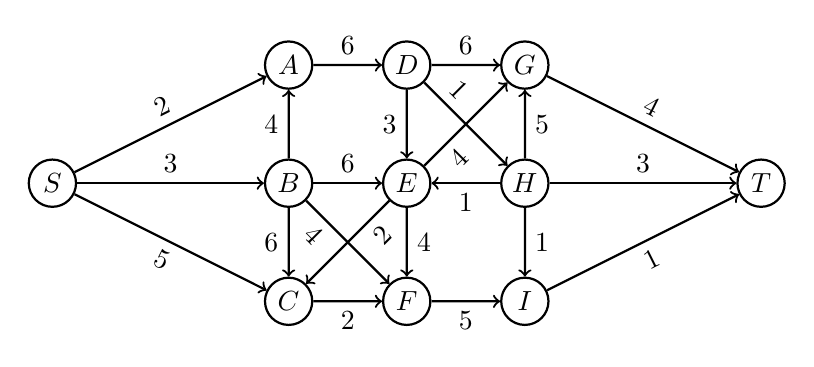
\begin{tikzpicture}[style=thick,scale=1.5]
\tikzstyle{every node}=[]
\tikzstyle{vertex}=[draw, circle, fill=white, inner sep=0pt, minimum size=6mm]

\node[vertex] (S) at ( 0, 0) {$S$};
\node[vertex] (A) at ( 2, 1) {$A$};
\node[vertex] (B) at ( 2, 0) {$B$};
\node[vertex] (C) at ( 2,-1) {$C$};
\node[vertex] (D) at ( 3, 1) {$D$};
\node[vertex] (E) at ( 3, 0) {$E$};
\node[vertex] (F) at ( 3,-1) {$F$};
\node[vertex] (G) at ( 4, 1) {$G$};
\node[vertex] (H) at ( 4, 0) {$H$};
\node[vertex] (I) at ( 4,-1) {$I$};
\node[vertex] (T) at ( 6,-0) {$T$};

\draw[->] (S) -- (A) node[midway, above, sloped] {$2$};
\draw[->] (S) -- (B) node[midway, above] {$3$};
\draw[->] (S) -- (C) node[midway, below, sloped] {$5$};
\draw[->] (A) -- (D) node[midway, above] {$6$};
\draw[->] (B) -- (A) node[midway, left] {$4$};
\draw[->] (B) -- (C) node[midway, left] {$6$};
\draw[->] (B) -- (E) node[midway, above] {$6$};
\draw[->] (B) -- (F) node[midway, near start, below, sloped] {$4$};
\draw[->] (C) -- (F) node[midway, below] {$2$};
\draw[->] (D) -- (E) node[midway, left] {$3$};
\draw[->] (D) -- (G) node[midway, above] {$6$};
\draw[->] (D) -- (H) node[midway, near start, above, sloped] {$1$};
\draw[->] (E) -- (C) node[midway, near start, below, sloped] {$2$};
\draw[->] (E) -- (F) node[midway, right] {$4$};
\draw[->] (E) -- (G) node[midway, near start, below, sloped] {$4$};
\draw[->] (F) -- (I) node[midway, below] {$5$};
\draw[->] (G) -- (T) node[midway, above, sloped] {$4$};
\draw[->] (H) -- (E) node[midway, below] {$1$};
\draw[->] (H) -- (G) node[midway, right] {$5$};
\draw[->] (H) -- (I) node[midway, right] {$1$};
\draw[->] (H) -- (T) node[midway, above] {$3$};
\draw[->] (I) -- (T) node[midway, below, sloped] {$1$};
\end{tikzpicture}
\podnaslov{Graf}
\end{slika}
\end{vprasanje}
\begin{odgovor}
\end{odgovor}
\end{naloga}


\begin{naloga}{Janoš Vidali}{Izpit OR 28.8.2018}
\begin{vprasanje}[pot]
Odpravljamo se na pot, ki bo trajala več dni.
Pripravili smo si seznam krajev in povezav med njimi,
ki jih lahko prevozimo v enem dnevu.
Za vsako povezavo poznamo stroške prevoza,
prav tako pa za vsak kraj poznamo še stroške nočitev.
Poiskati želimo čim cenejšo pot od začetne točke do destinacije
(tj., skupna cena prevozov in nočitev naj bo čim manjša).

\begin{enumerate}[(a)]
\item Predstavi problem v jeziku grafov
in predlagaj čim bolj učinkovit algoritem za njegovo reševanje.

\item S pomočjo zgornjega algoritma poišči najcenejšo pot od LJ do BX
v grafu s slike~\fig{pocitnice}.
Na povezavah so napisani stroški prevozov med krajema
(veljajo za obe smeri),
pri vozliščih pa stroški prenočitve v kraju.
\end{enumerate}
\end{vprasanje}
\begin{odgovor}
\end{odgovor}
\end{naloga}
